% !TeX spellcheck = de_DE
\section{Finite Differenzen Methode}
	Als Beispiel sei das elektrische Skalarpotential $V$ eines Zylinderkondensators zu bestimmen, also das Lösen der Differentialgleichung:
	\begin{equation}
	-\frac{1}{r} \frac{\partial}{\partial r} ( r \frac{\partial }{\partial r} u(r)) = 0
	\end{equation}
	was dem elektrischen Skalarpotential entspricht.
	\begin{equation}
		\vec \nabla \cdot \epsilon_0 \vec \nabla V = 0
		\label{e-potential}
	\end{equation}
	Aufgrund der Symmetrie - es wird passenderweise ein Zylinderkoordinatensystem gewählt - kann das Problem eindimensional betrachtet werden, also:
	\begin{equation}
	V(r,\phi, z) = V(r)
	\end{equation}
	Als Randbedingung sind $V(r=1)=0$ und $V(r=5)=100$ vorgegeben. 
	\\
	
	{\Large Aufgaben \par}
	\begin{enumerate}
		\item Bestimmen Sie die analytische Lösung $u(r)$.
		\item Bestimmen Sie eine numerische Lösung mittels Methode der finiten Differenzen indem Sie das Intervall (1,5) gleichmäßig in 4 Teilintervalle teilen und den Differentialoperator diskretisieren.
		\item  Vergleichen Sie die analytische Lösung mit der numerischen Lösung. Wie groß ist der relative Fehler in \% in den Knotenpunkten?
	\end{enumerate}
	
	
	\subsection{Analytische Lösung}
	Die Differentialgleichung kann analytisch gelöst werden. Hierzu wird zuerst das erste Differenzial aufgelöst und die Gleichung auf folgende Form gebracht:
	\begin{equation}
	\frac{1}{r} \frac{\partial }{\partial r} u(r) +  \frac{\partial^2}{\partial r^2} u(r) = 0
	\end{equation}
	umformen und integrieren:
	\begin{eqnarray}
		-\frac{1}{r} \frac{\partial}{\partial r} ( r \frac{\partial }{\partial r} u(r)) = 0 \\
		 \frac{\partial}{\partial r} ( r \frac{\partial }{\partial r} u(r)) = 0 \\
		  r \frac{\partial }{\partial r} u(r) = C_1 \\
		  \frac{\partial }{\partial r} u(r) = \frac{C_1}{r} \\
	\end{eqnarray}
	
%	Wir wissen, wie die Lösung ungefähr auszusehen hat, nämlich in etwa die Form $u=C r^\lambda$ haben wird. Wir können also also diesen allgemeinen Ansatz wählen und in die Gleichung einsetzen (dabei wurden die konstanten Faktoren gleich gekürzt).
%	Das führt dann auf:
%	\begin{equation}
%	\lambda \frac{1}{r} r^{\lambda-1} + \lambda^2 r^{\lambda -2} = 0
%	\end{equation}
%	Wie leicht zu erkennen ist, können auch die $r$'s gekürzt werden und anschließend $\lambda$ bestimmt werden. Mit
%	\[
%	\lambda_1 = 0 , \quad \lambda_2 = -1
%	\]	
%	erhalten wir nun als allgemeine Lösung unserer homogenen Differentialgleichung
%	\begin{equation}
%	u(r) = C_1 r^{\lambda_1} + C_2 r^{\lambda_2} = C_1 + C_2 \frac{1}{r}
%	\end{equation}
%	mit noch zu bestimmenden Konstanten $C_1$ und $C_2$. Diese werden so gewählt, dass die Lösung unsere Randbedingungen erfüllt. Für $u(1) = 0$ ergibt sich:
%	\begin{equation}
%	u(1)=C_1 + C_2 = 0 \quad \Rightarrow \quad C_1 = - C_2
%	\end{equation}
%	Und für die zweite Randbedingung ergibt sich (für $C_2$ wurde gleich $-C_1$ eingesetzt):
%	\begin{equation}
%	u(5)=C_1 - C_1 \frac{1}{5} = 100 \quad \Rightarrow \quad C_1 = -125
%	\end{equation}
	
	Nochmaliges integrieren nach $r$ bringt uns schließlich auf
	\begin{equation}
	u(r)= 	\int \frac{\partial u}{\partial r} dr = C_1 \ln r + C_2
	\end{equation}
	mit noch zu bestimmenden Konstanten $C_1$ und $C_2$. Diese werden so gewählt, dass die Lösung unsere Randbedingungen erfüllt. Für $u(1) = 0$ ergibt sich:
	\begin{equation}
	u(1)=C_1 \ln(1) + C_2 =  0 \quad \Rightarrow \quad C_2 = 0
	\end{equation}
	Und für die zweite Randbedingung ergibt sich:
	\begin{equation}
	u(5)=C_1 \ln(5)  = 100 \quad \Rightarrow \quad C_1 =\frac{100}{\ln 5} \approx 62.13349...
	\end{equation}
	\\
	

	
	\subsection{Numerische Lösung}
	Für die nummerische Berechnung wurde das Intervall in 4 Teilintervalle aufgeteilt und jeweils das Potential an den Stützstellen $r=\{1,2,3,4,5\}$ berechnet.	Die Gleichung \ref{e-potential} ist ausgeschrieben und in Zylinderkoordinaten:
	\begin{equation}
	-\frac{1}{r} \frac{\partial}{\partial r} ( r \frac{\partial }{\partial r} u(r)) = 0
	\end{equation}
	Durch Anwenden der Produktregel lässt sich das Gleichgungssystem auf 
	\begin{equation}
	\frac{1}{r} \frac{\partial}{\partial r} ( r \frac{\partial }{\partial r} u(r)) = \frac{1}{r} \frac{\partial }{\partial r} u(r) +  \frac{\partial^2}{\partial r^2} u(r) = 0
	\end{equation}
	Da wir $u(r=1)=0$ und $u(r=5)=100$ bereits kennen, konstruieren wir einen Vektor mit den gesuchten Werten der Knotenpunkte $2,3,4$:
	\begin{equation}
	\mathbf{u} =	\begin{bmatrix}
	u_2\\
	u_3\\
	u_4
	\end{bmatrix}
	\end{equation}
	Das Differential wird numerisch mit dem zentralen Differenzen Quotient angenähert:
	\begin{equation}
	\frac{\partial u(r)}{\partial r} \approx \frac{u(r+h)-u(r-h)}{2 h}
	\end{equation}
	und entsprechend für die zweite Ableitung wurde
	\begin{equation}
		\frac{\partial^2 u(r)}{\partial r^2} \approx \frac{u(r+h)-2u(r)+u(r-h)}{h^2}
	\end{equation}
	gewählt. Die Herleitung erfolgt über die Taylorreihen-Entwicklung.
	
	Wir konstruieren unser lineares Gleichungssystem folgendermaßen:
	\begin{equation}
	\frac{1}{2rh} \mathbf{A} \mathbf{u} + \frac{1}{h^2}\mathbf{B}  \mathbf{u} = \mathbf{f}
	\end{equation}
	wobei die Matrizen $\mathbf{A}$ und $\mathbf{B}$ die Koeffizienten für die Differnezenquotienten enthalten. Der Vektor $\mathbf{f}$ enthält die rechte Seite der Differenzialgleichung (die hier allerdings immer 0 ist) und außerdem die entsprechenden Randbedingungen die zum Lösen erforderlich sind.
	\begin{equation}
	\mathbf{f} = \begin{bmatrix}
	\frac{1}{rh} u_1  - \frac{1}{h^2} u_1 \\
	0 \\
	-\frac{1}{2rh} u_5  - \frac{1}{h^2} u_5 
	\end{bmatrix}
	\end{equation}
	Ausgeschrieben erhält man mit $h=1$ und $r=\{2,3,4\}$:
	\begin{equation}
	\frac{1}{2}
	\begin{bmatrix}
	0 & \frac{1}{2} & 0 \\ 
	-\frac{1}{3} & 0 & \frac{1}{3} \\ 
	0 & -\frac{1}{4} & 0
	\end{bmatrix}   
	\begin{bmatrix}
	u_2\\
	u_3\\
	u_4
	\end{bmatrix} +   \begin{bmatrix}
	-2 & 1 & 0 \\ 
	1 & -2 & 1 \\ 
	0 & 1 & -2
	\end{bmatrix}  \begin{bmatrix}
	u_2\\
	u_3\\
	u_4
	\end{bmatrix} = \begin{bmatrix}
	\frac{1}{2} u_1  -  u_1 \\
	0 \\
	-\frac{1}{8} u_5  -  u_5 
	\end{bmatrix}
	\end{equation}
	Die Matrizen können leicht zusammengefasst werden und anschließend gelöst werden.


	\subsection{Implementierung in Matlab}
	\lstinputlisting[language=matlab,style=myMatlabStyle,caption={Implementierung der FDM für die Berechnung des Potenzials in einem Zylinderkondensators. Eine Anpassung der Anzahl der Stützstellen ist möglich über die Variable $N$}]{../Matlab/FDM.m}
	
	\subsection{Ergebnisse}
	
	Die Methode der finiten Differenzen erlaubt eine zuverlässige Berechnung einer einfachen Differentialgleichung. Der relative Fehler ist selbst bei wenigen Stützstellen sehr gering.
		
	\begin{figure}[!h]
		\centering
	\begin{tabular}{cc}
		\begin{subfigure}{0.45\linewidth}
			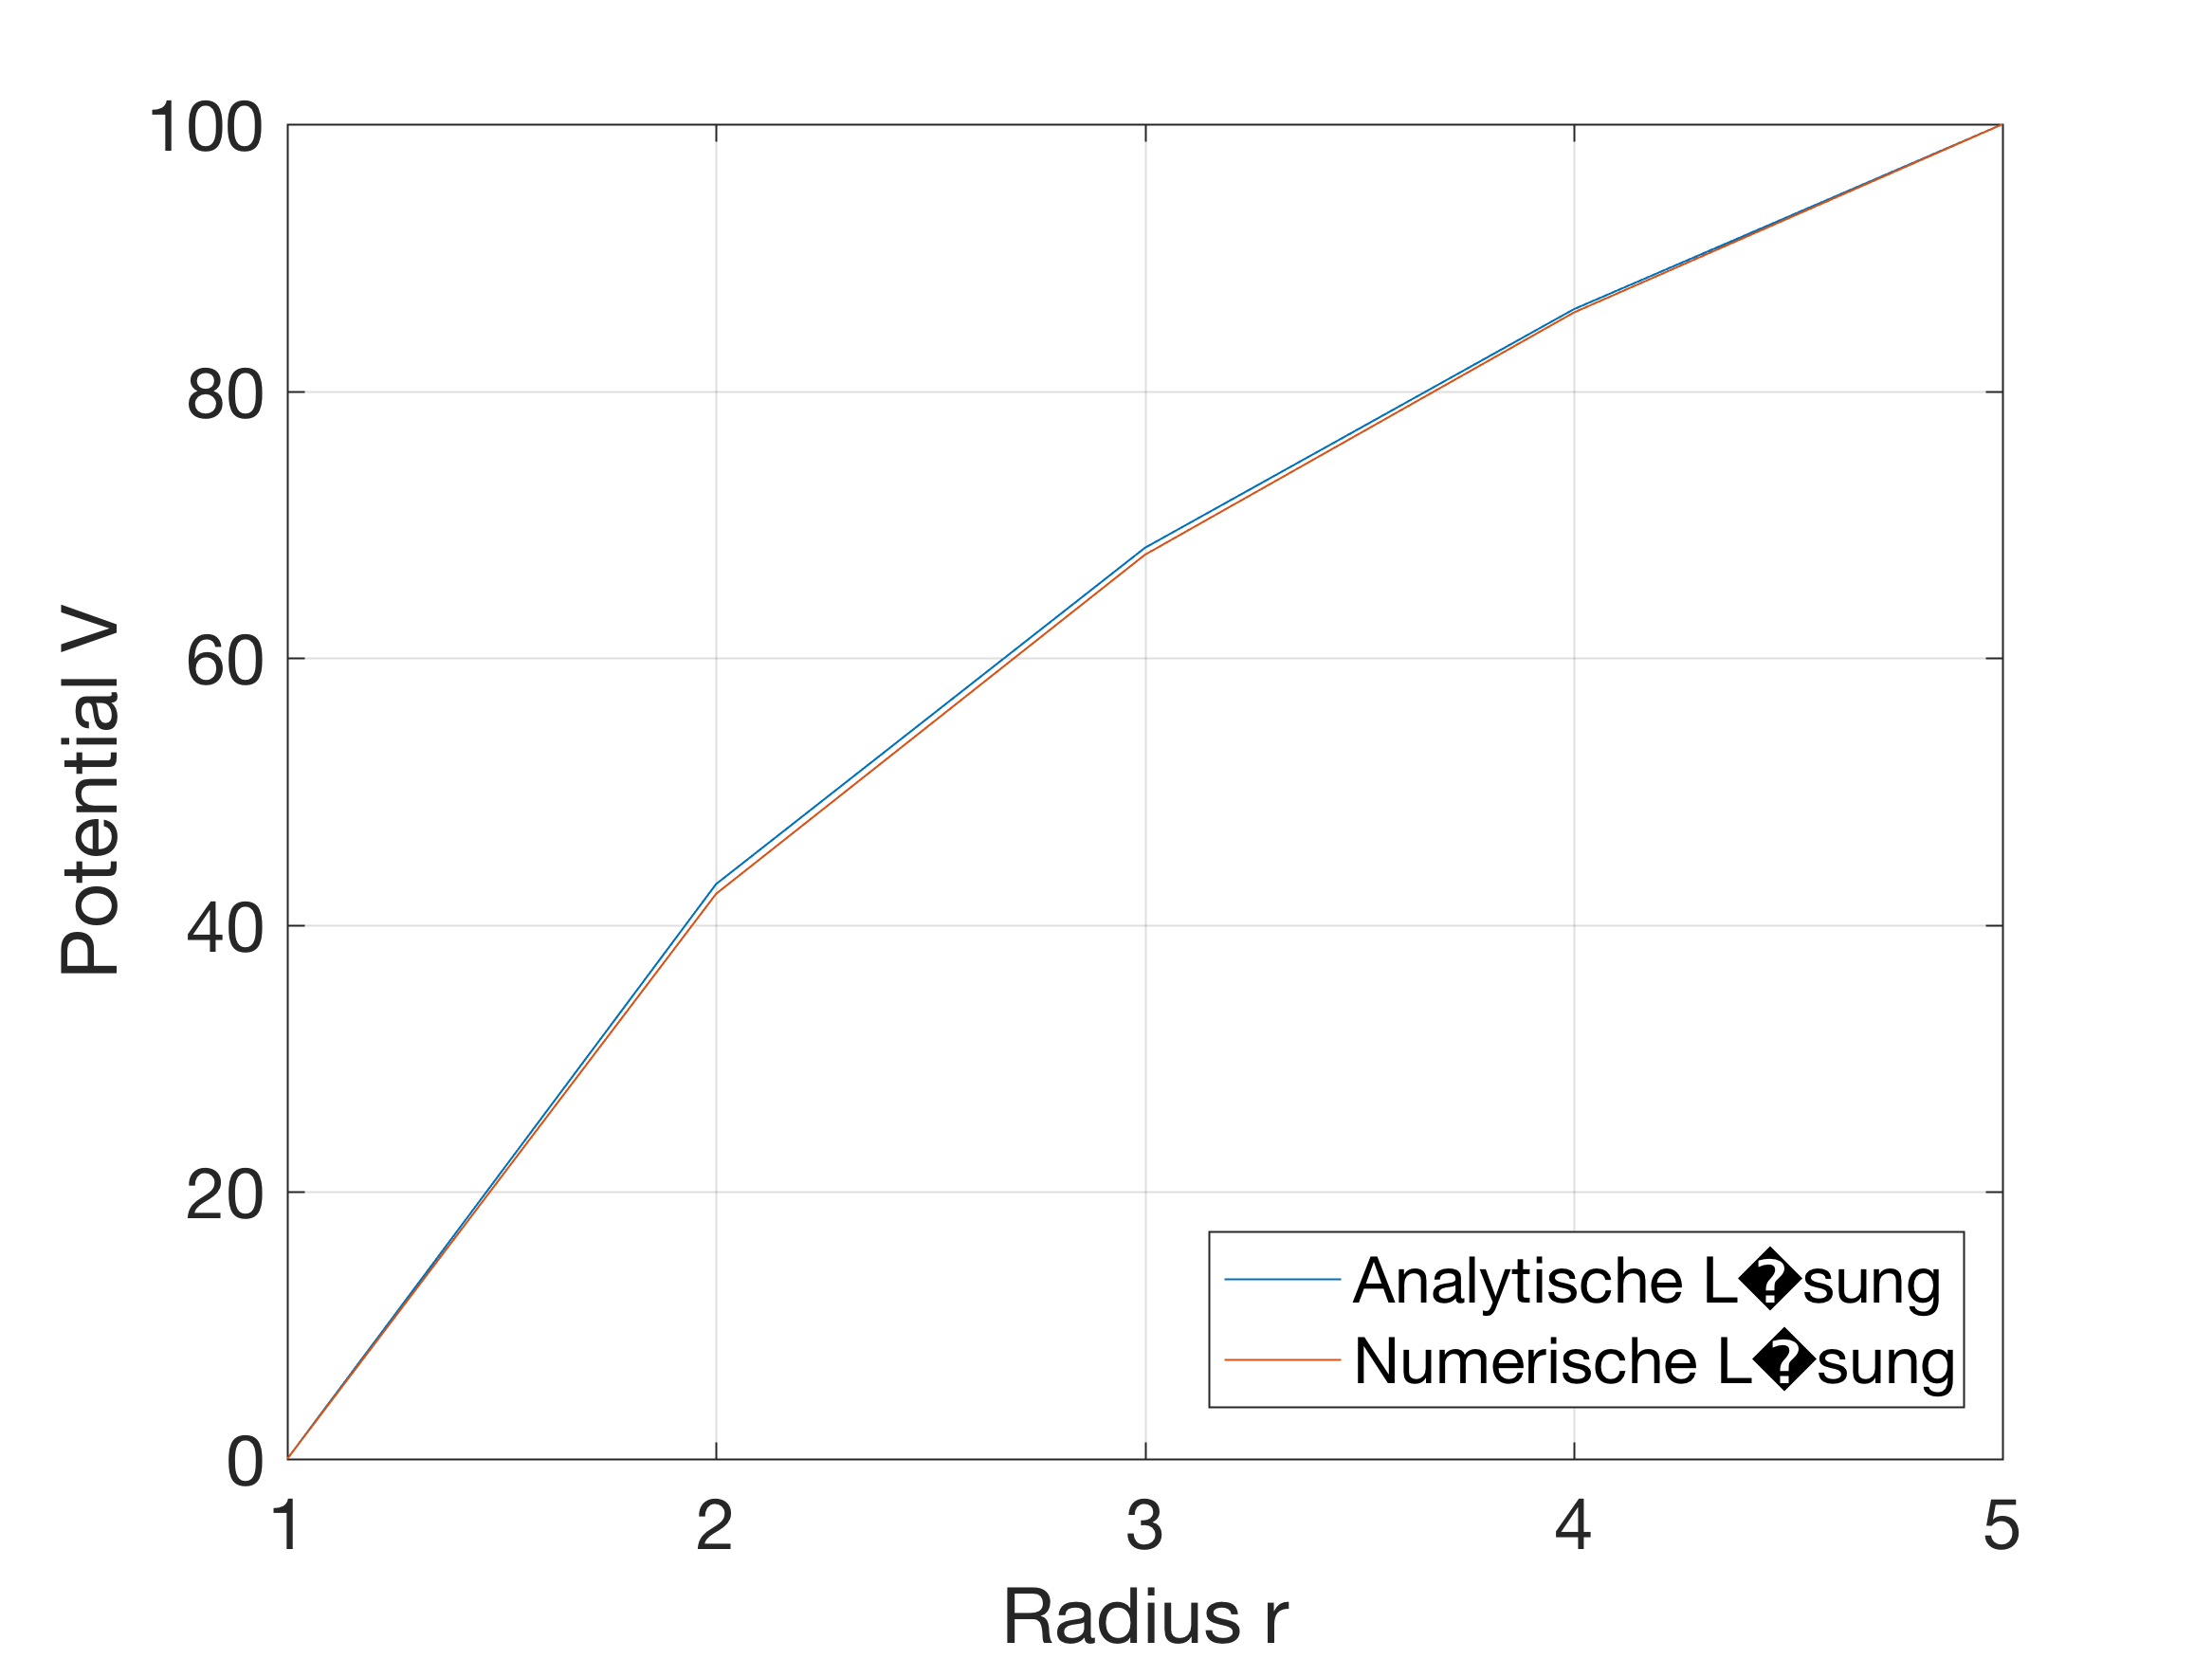
\includegraphics[width=\linewidth]{../Matlab/cylinder}
			\caption{Plot}
			\label{fig:cylinder}
		\end{subfigure}
		~
		\begin{subfigure}{0.45\linewidth}
			
			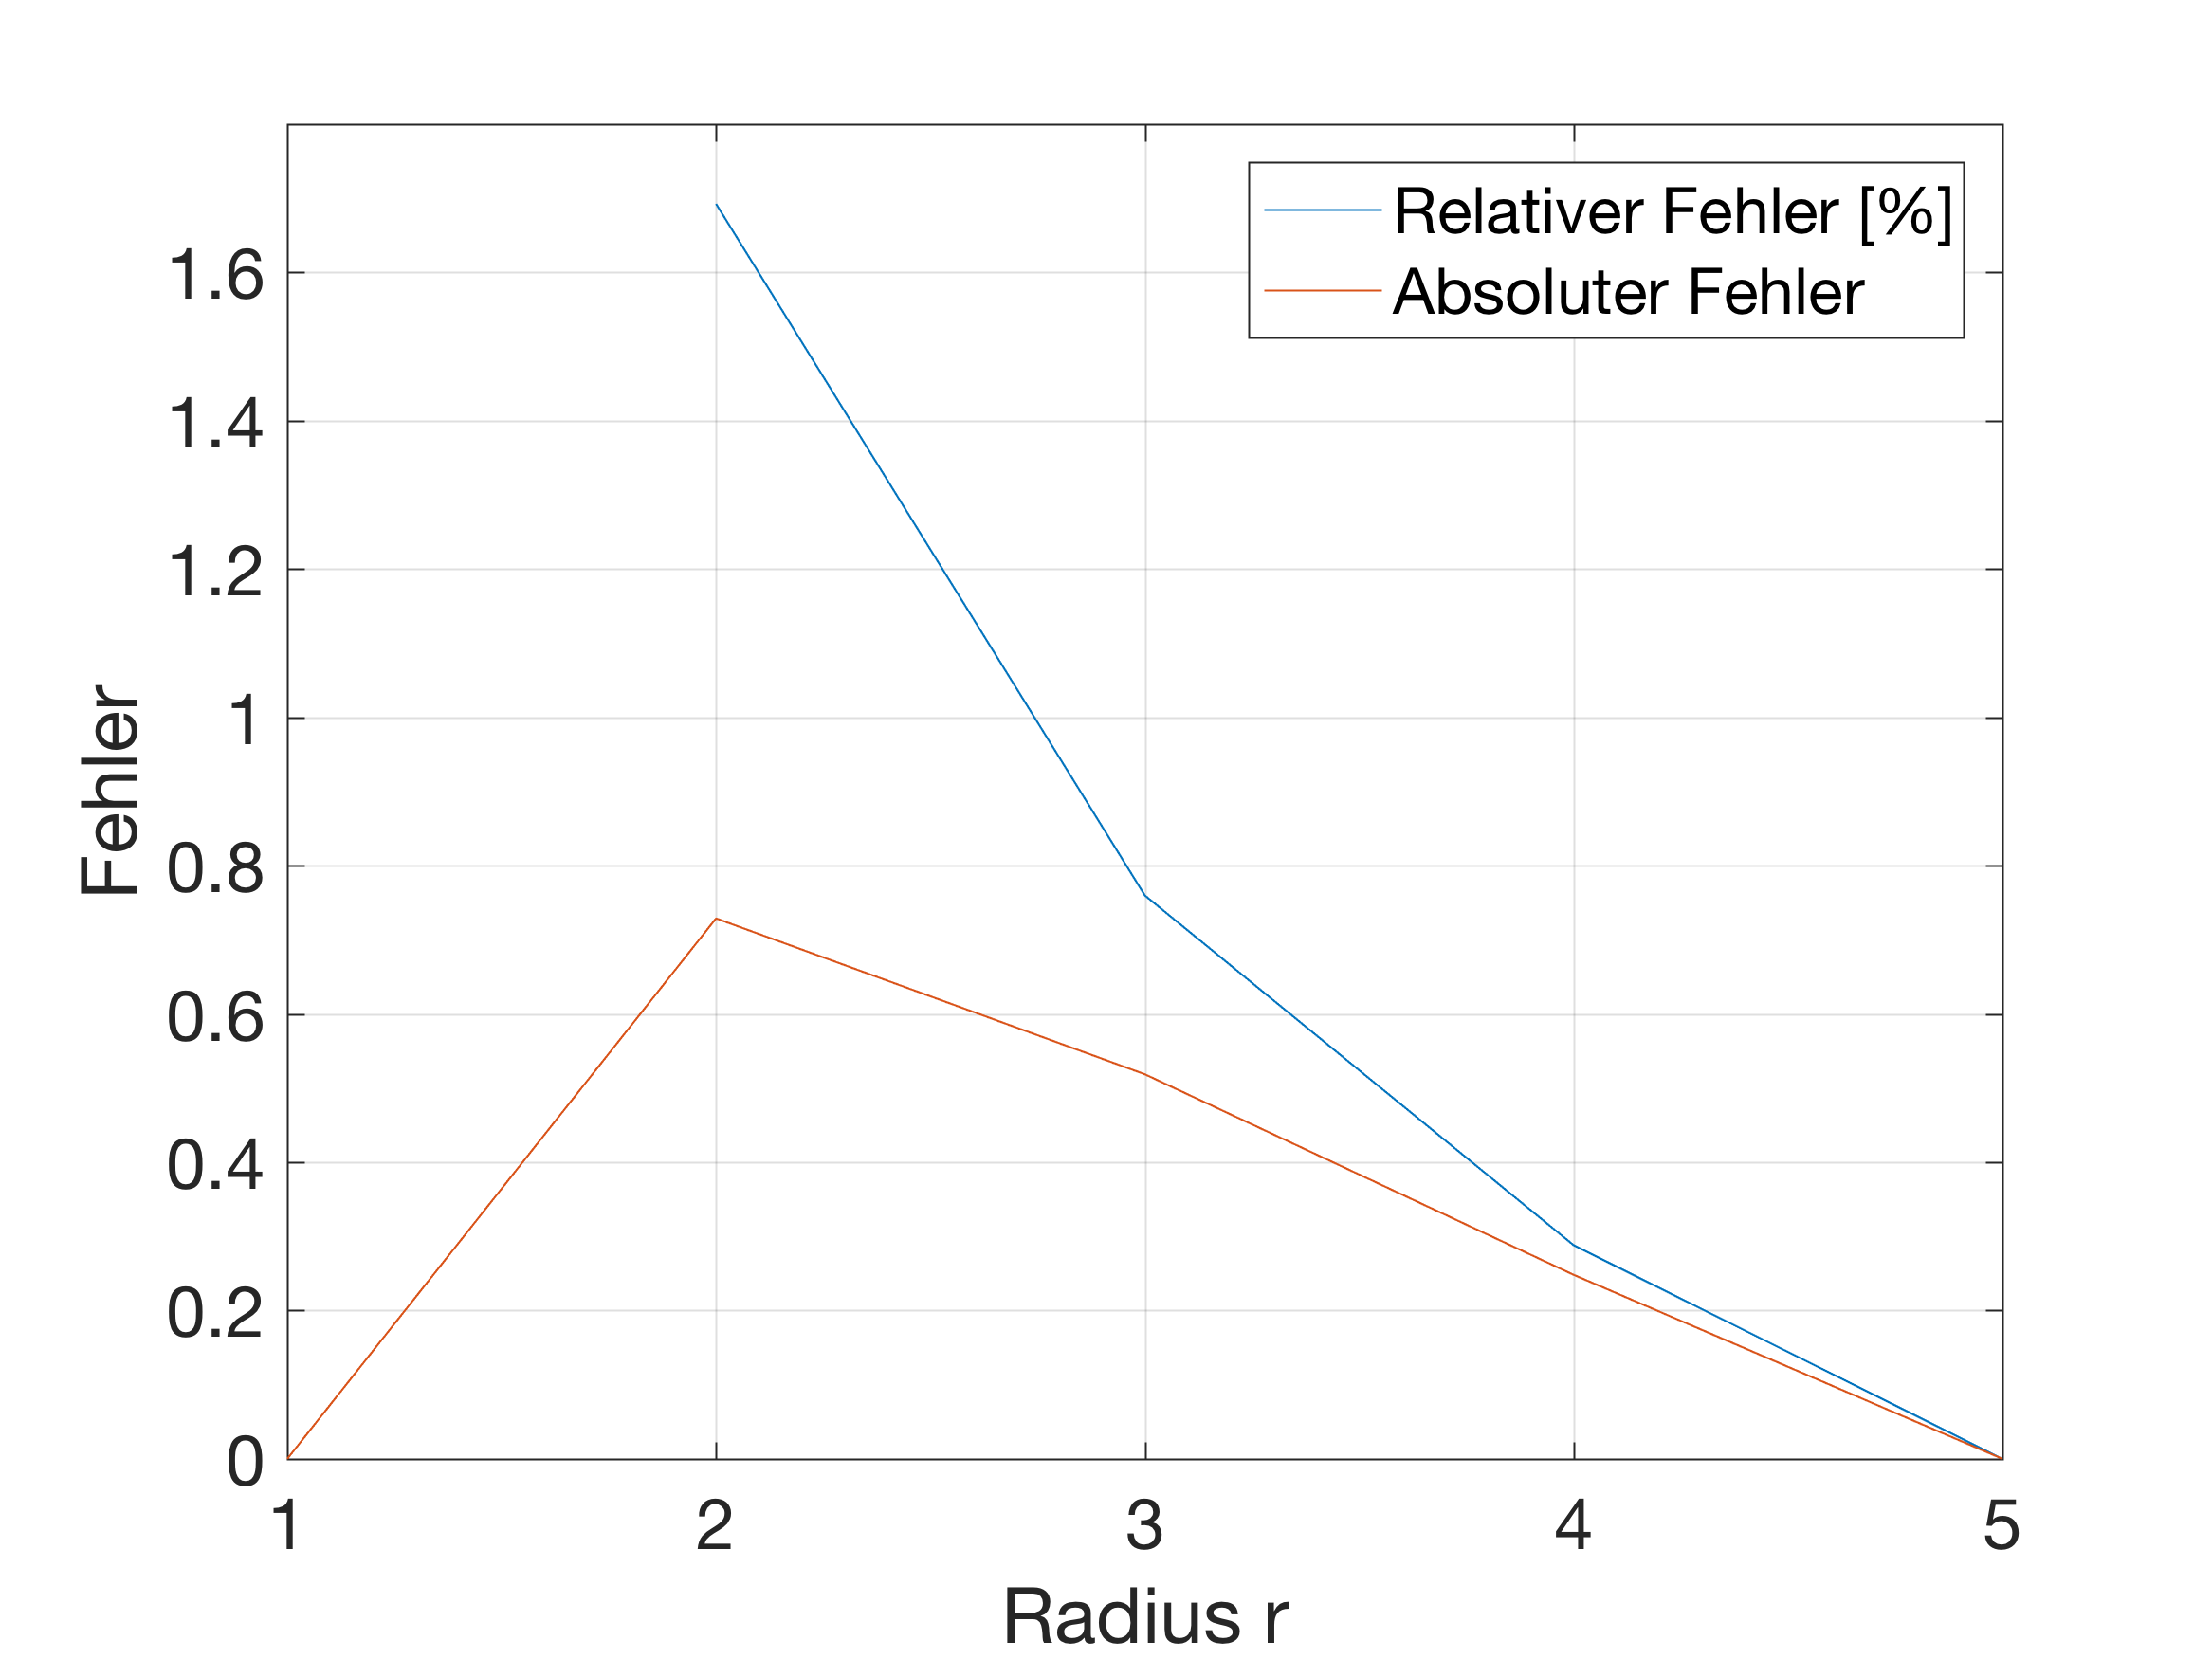
\includegraphics[width=\linewidth]{../Matlab/error}
			\caption{Error}
			\label{fig:error}
		\end{subfigure}
		
	\end{tabular}
	\caption{Ergebnisse für 3 Stützstellen im Intervall $r=[1,5]$}
	\end{figure}

	\begin{table}[!h]
	\centering
	\caption{Ergebnisse der FDM für $N=3$}
	\begin{tabular}{|c|c|c|c|}
		\hline 
		&  Analytisch & Numerisch & Relativer Fehler [\%] \\ 
		\hline 
		$u_2$ & 43.0677 & 42.3387 & 1.6926 \\ 
		\hline 
		$u_3$ & 68.2606 & 67.7419 & 0.7599 \\ 
		\hline 
		$u_4$ & 86.1353 & 85.8871 & 0.2882 \\ 
		\hline 
	\end{tabular} 

  



	
	\end{table}